\documentclass[cn,10pt,math=newtx,citestyle=gb7714-2015,bibstyle=gb7714-2015]{elegantbook}

%latex 宏
% 书签
\usepackage{bookmark}
% 画图
\usepackage{tikz}
% 图片
\usepackage{graphicx}
\usepackage{caption}
\usepackage{subfigure}
\usepackage{float}

%region 元数据声明
\title{ \LaTeX{} 入门手册}
\subtitle{快速入门 \LaTeX{} 文档编写}

\author{igrape}
\institute{TropicalTeamYard}
\date{2021年7月2日}
\version{0.1}

\extrainfo{各人自扫门前雪,休管他人瓦上霜。—— 陈元靓}

\setcounter{tocdepth}{3}

\cover{images/cover.jpg}


%endregion
\begin{document}
    \maketitle

    \frontmatter

    \chapter*{特别声明}

    \markboth{Introduction}{前言}

    在2019年4月6日我便写过一个 \LaTeX{} 入门的文档,因此可以说我对 \LaTeX{} 还是有一定了解的,然而在一段时间没有接触 \LaTeX{} 之后,我对 \LaTeX{} 的语法就非常生疏了。因此编写一个类似于 \LaTeX{} 相关的入门手册还是很有必要的。因为我发现,无论是从环境的搭建,\LaTeX{} 语法的学期,文档的编写,都存在一定的难度。
    \vskip 0.5cm
    
    另外,此文档将会逐渐整合我之间写的东西,并在此基础上进行更新。
    
    \vskip 0.5cm
    

    \begin{flushright}
    igrape \\
    2021年7月2日
    \end{flushright}
    
    \tableofcontents

    \mainmatter

    \chapter{\LaTeX{} 的环境配置}

    \begin{flushright}
        \begin{tikzpicture}
            \draw (0,0) node [fill=red!30!white] {2021年7月3日};
        \end{tikzpicture}
    \end{flushright}

    \section{TexLive的安装
        \footnote{参考自知乎教程\textbf{LaTeX:TeXLive2021安装}:\quad\url{https://zhuanlan.zhihu.com/p/362201376}}
    }

    \subsection{TexLive下载}

    

    TexLive是使用Tex环境的最关键的软件之一,其作用相当于SDK,是编译\LaTeX{}必须的环境。因此如果你要在本地使用\LaTeX{}套装,你就有必要安装TexLive。推荐安装TexLive的最新发行版。你可以到\href{http://www.tug.org/texlive/}{TexLive官网}下载镜像文件,也可以到其他的开源镜像站下载镜像文件。如果要查看更多的镜像源列表,可以到\href{https://ctan.org/mirrors}{CTAN Sites}查看。

    \begin{table}[htbp]
        \centering
        \caption{TexLive 常用的TexLive镜像源}
        \begin{tabular}{p{0.20\textwidth}p{0.60\textwidth}}
            \toprule
                镜像源 & 地址 \\
            \midrule    
                utsc & \url{https://mirrors.ustc.edu.cn/CTAN/systems/texlive/Images/} \\
                aliyun(阿里云) & \url{https://mirrors.aliyun.com/CTAN/systems/texlive/Images/} \\
                tsinghua(清华大学) & \url{https://mirrors.tuna.tsinghua.edu.cn/CTAN/systems/texlive/Images/} \\
            \bottomrule
        \end{tabular}
    \end{table}

    \textbf{官网下载流程:}

    1. 打开\href{http://www.tug.org/texlive/}{TexLive官网},点击\textbf{on DVD}。

    \begin{figure}[H]
        \centering
        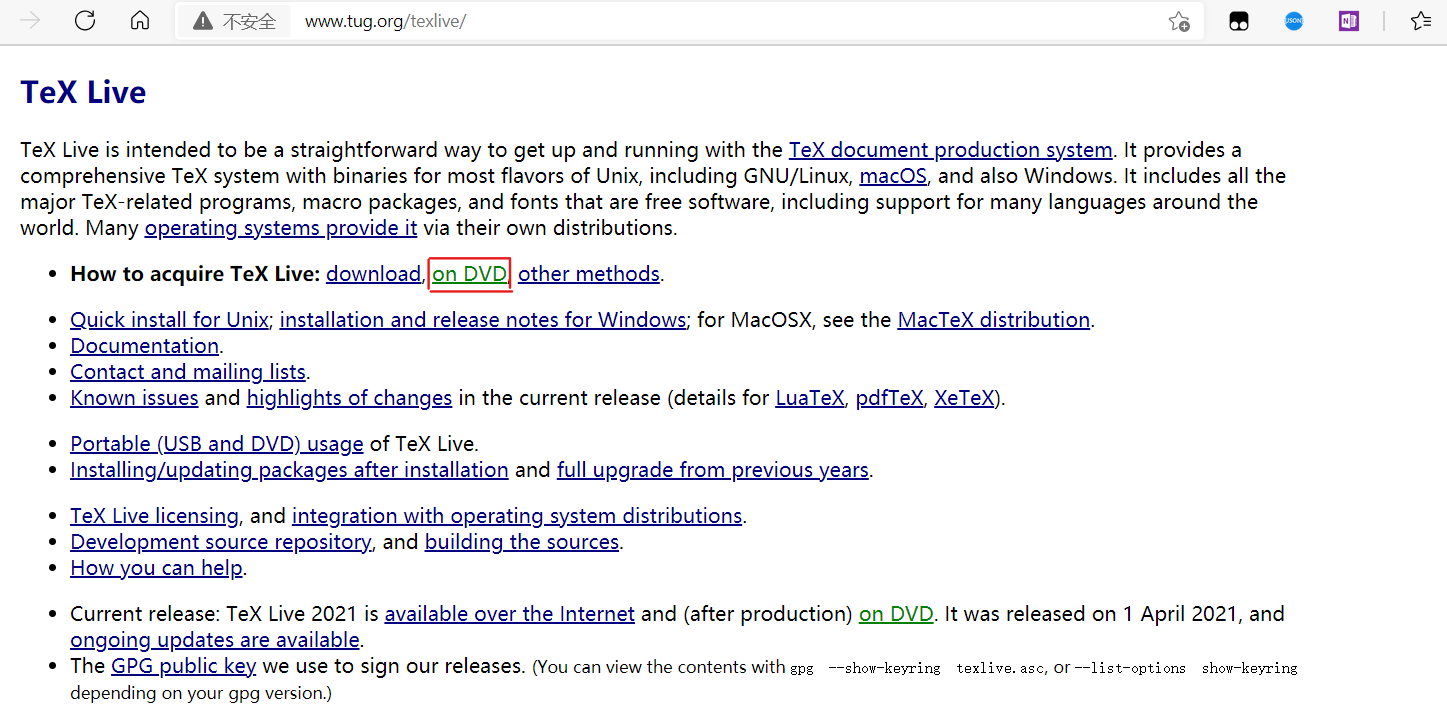
\includegraphics[width=0.8\textwidth]{images/shapshot_install_1.png}
        \caption{TexLive官网}
        \label{shapshot_install_1}
    \end{figure}
    
    2. 跳转后选择红框的链接

    \begin{figure}[H]
        \centering
        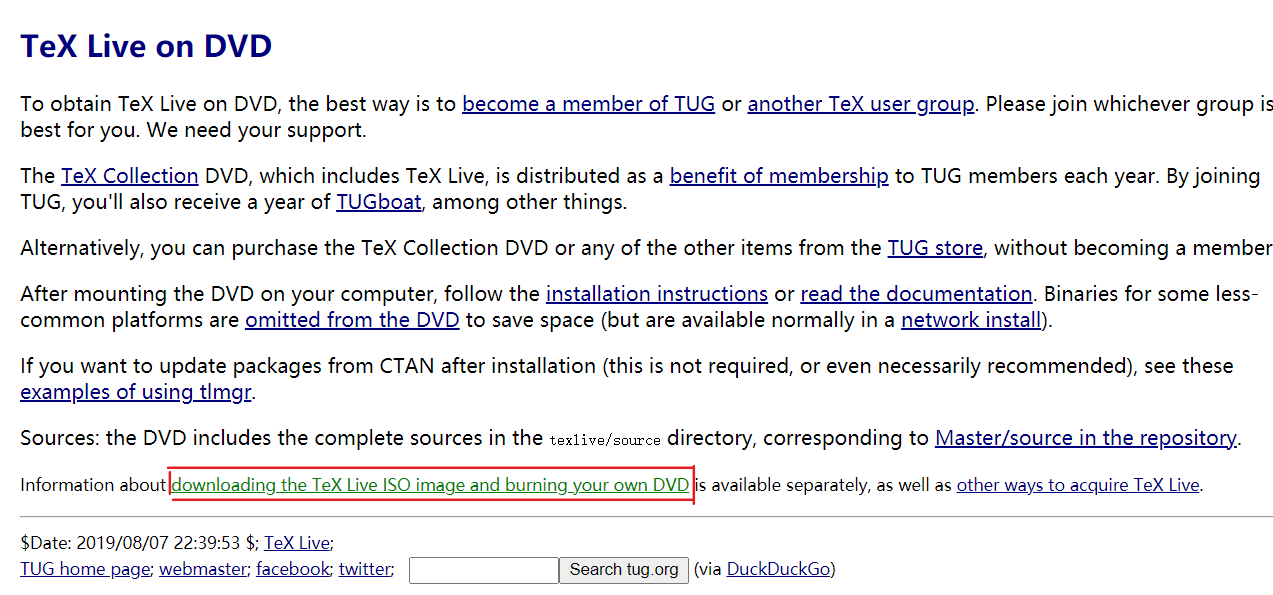
\includegraphics[width=0.8\textwidth]{images/shapshot_install_2.png}
        \caption{TexLive官网}
        \label{shapshot_install_2}
    \end{figure}

    3. 选择\textbf{download from a nearby CTAN mirror}

    \begin{figure}[H]
        \centering
        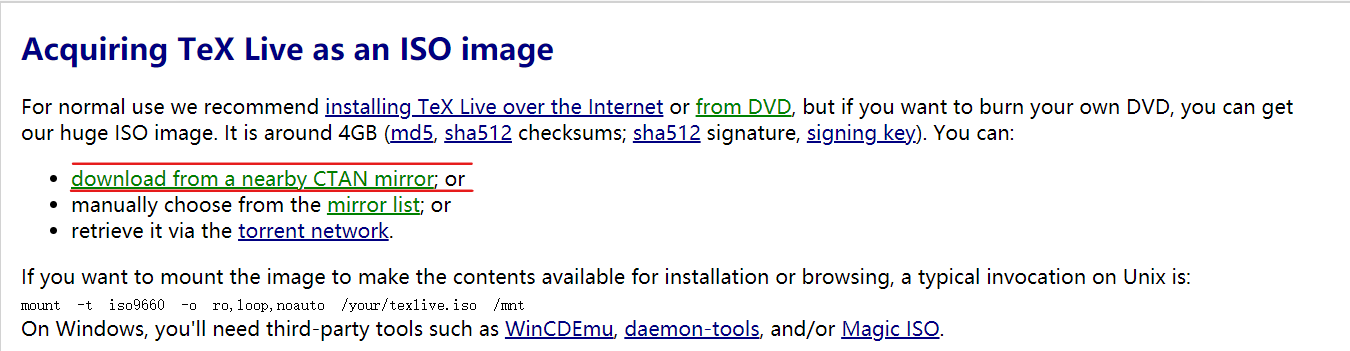
\includegraphics[width=0.8\textwidth]{images/shapshot_install_3.png}
        \caption{TexLive官网}
        \label{shapshot_install_3}
    \end{figure}

    \begin{note}
        安装TexLive到本地是一个比较费时的过程,如果你只是想要体验或者\LaTeX{}语法的话,你也可以到\href{https://www.overleaf.com/}{Overleaf官网}学习和使用。
    \end{note}

    然后等待TexLive镜像文件下载完成

    \subsection{TexLive 安装}

    \subsection{vscode环境配置}

    \subsection{开始编写第一个\LaTeX{}项目}

    \chapter{\LaTeX{} 语法介绍}

    \section{\LaTeX{} 宏}

    \subsection{\LaTeX{} 宏命令}

    \subsection{\LaTeX{} 宏环境}

    \subsection{\LaTeX{} 宏包}
    
    \section{\LaTeX{} 字符}

    \subsection{\LaTeX{} 转义字符}

    \subsection{\LaTeX{} 符号}

    \subsection{\LaTeX{} 使用表情符号}

    \section {文档格式}

    \subsection {报告(Paper)}

    \subsection {书籍(Book)}

    \section {内容与段落}

    \subsection {标题或封面}

    \subsection {段落}

    \subsection {导入文档片段}

    \subsection {目录}

    \subsection {对齐}

    \subsection {中文字符支持}

    \section {页面布局}

    \section {文字效果}

    \subsection {加粗、倾斜等常用文字效果}

    \subsection {字体}

    \subsection {着重号}

    \subsection {首字下沉}

    \subsection {强调色}

    \section {颜色}

    \section {媒体内容}
    
    \subsection {传统表格}

    \subsection {多表格}
    
    \subsection {公式}

    \subsection {绘图(TikZ)}

    \subsection {代码块}

    \subsection {链接}

    \subsection {书签}

    \subsection {注解}

    \section {引用}
    

    

    \chapter{代码块}

    \chapter{\LaTeX{} 公式}

    \chapter{\LaTeX{} 样式}

    \section {Elegant \LaTeX{} 介绍}

    \chapter{\LaTeX{}编译}

    \chapter{TikZ绘图工具}

    \chapter{常见Q\&A}



\end{document}